% This template has been tested with LLNCS DOCUMENT CLASS -- version 2.20 (24-JUN-2015)

%"runningheads" enables:
%  - page number on page 2 onwards
%  - title/authors on even/odd pages
%This is good for other readers to enable proper archiving among other papers and pointing to content.
%Even if the title page states the title, when printed and stored in a folder, when blindly opening the folder, one could hit not the title page, but an arbitrary page. Therefore, it is good to have title printed on the pages, too.
\documentclass[runningheads,a4paper]{llncs}[2015/06/24]

%Even though `american`, `english` and `USenglish` are synonyms for babel package (according to https://tex.stackexchange.com/questions/12775/babel-english-american-usenglish), the llncs document class is prepared to avoid the overriding of certain names (such as "Abstract." -> "Abstract" or "Fig." -> "Figure") when using `english`, but not when using the other 2.
\usepackage[english]{babel}

%better font, similar to the default springer font
%cfr-lm is preferred over lmodern. Reasoning at http://tex.stackexchange.com/a/247543/9075
\usepackage[%
rm={oldstyle=false,proportional=true},%
sf={oldstyle=false,proportional=true},%
tt={oldstyle=false,proportional=true,variable=true},%
qt=false%
]{cfr-lm}
%
%if more space is needed, exchange cfr-lm by mathptmx
%\usepackage{mathptmx}

\usepackage{graphicx}


%% If you need packages for other papers,
%% START COPYING HERE

%extended enumerate, such as \begin{compactenum}
\usepackage{paralist}

\usepackage{amsmath}
%put figures inside a text
%\usepackage{picins}
%use
%\piccaptioninside
%\piccaption{...}
%\parpic[r]{\includegraphics ...}
%Text...

%Sorts the citations in the brackets
%It also allows \cite{refa, refb}. Otherwise, the document does not compile.
%  Error message: "White space in argument"
\usepackage{cite}

\usepackage[T1]{fontenc}
\usepackage{cmap}

%for demonstration purposes only
\usepackage[math]{blindtext}

%for easy quotations: \enquote{text}
\usepackage{csquotes}

%enable margin kerning
\usepackage{microtype}

%tweak \url{...}
\usepackage{url}
\urlstyle{same}
%improve wrapping of URLs - hint by http://tex.stackexchange.com/a/10419/9075
\makeatletter
\g@addto@macro{\UrlBreaks}{\UrlOrds}
\makeatother
%nicer // - solution by http://tex.stackexchange.com/a/98470/9075
%DO NOT ACTIVATE -> prevents line breaks
%\makeatletter
%\def\Url@twoslashes{\mathchar`\/\@ifnextchar/{\kern-.2em}{}}
%\g@addto@macro\UrlSpecials{\do\/{\Url@twoslashes}}
%\makeatother

%diagonal lines in a table - http://tex.stackexchange.com/questions/17745/diagonal-lines-in-table-cell
%slashbox is not available in texlive (due to licensing) and also gives bad results. This, we use diagbox
%\usepackage{diagbox}

%required for pdfcomment later
\usepackage{xcolor}

% new packages BEFORE hyperref
% See also http://tex.stackexchange.com/questions/1863/which-packages-should-be-loaded-after-hyperref-instead-of-before

%enable hyperref without colors and without bookmarks
\usepackage[
%   pdfauthor={},
%   pdfsubject={},
%   pdftitle={},
%   pdfkeywords={},
   bookmarks=false,
   colorlinks=true,
   allcolors=black,
   pdfstartview=Fit,
   breaklinks=true,
]{hyperref}
%enables correct jumping to figures when referencing
\usepackage[all]{hypcap}

%enable nice comments
\usepackage{pdfcomment}
\newcommand{\commentontext}[2]{\colorbox{yellow!60}{#1}\pdfcomment[color={0.234 0.867 0.211},hoffset=-6pt,voffset=10pt,opacity=0.5]{#2}}
\newcommand{\commentatside}[1]{\pdfcomment[color={0.045 0.278 0.643},icon=Note]{#1}}

%compatibality with packages todo, easy-todo, todonotes
\newcommand{\todo}[1]{\commentatside{#1}}
%compatiblity with package fixmetodonotes
\newcommand{\TODO}[1]{\commentatside{#1}}

%enable \cref{...} and \Cref{...} instead of \ref: Type of reference included in the link
\usepackage[capitalise,nameinlink]{cleveref}
%Nice formats for \cref
\crefname{section}{Sect.}{Sect.}
\Crefname{section}{Section}{Sections}

\usepackage{xspace}
%\newcommand{\eg}{e.\,g.\xspace}
%\newcommand{\ie}{i.\,e.\xspace}
\newcommand{\eg}{e.\,g.,\ }
\newcommand{\ie}{i.\,e.,\ }

%introduce \powerset - hint by http://matheplanet.com/matheplanet/nuke/html/viewtopic.php?topic=136492&post_id=997377
\DeclareFontFamily{U}{MnSymbolC}{}
\DeclareSymbolFont{MnSyC}{U}{MnSymbolC}{m}{n}
\DeclareFontShape{U}{MnSymbolC}{m}{n}{
    <-6>  MnSymbolC5
   <6-7>  MnSymbolC6
   <7-8>  MnSymbolC7
   <8-9>  MnSymbolC8
   <9-10> MnSymbolC9
  <10-12> MnSymbolC10
  <12->   MnSymbolC12%
}{}
\DeclareMathSymbol{\powerset}{\mathord}{MnSyC}{180}

% correct bad hyphenation here
\hyphenation{op-tical net-works semi-conduc-tor}


%% END COPYING HERE


\begin{document}

\title{Implementation of a Brute Force Attack on the A5/1 Keystream Generator
in a GPU-based Volunteer Computing Project}
\titlerunning{Brute Force Attack on A5/1}

%Single insitute
\author{Vadim Bulavintsev \and Alexander Semenov \and Oleg Zaikin}
\authorrunning{Vadim Bulavintsev et al.}
\institute{Matrosov Institute for System Dynamics and Control Theory of
Siberian Branch of Russian Academy of Sciences, Irkutsk, Russia
\email{ichorid@mail.ru, biclop.rambler@yandex.ru, zaikin.icc@gmail.com}}

%Multiple insitutes
%Currently disabled
%
\iffalse
%Multiple institutes are typeset as follows:
\author{Firstname Lastname\inst{1} \and Firstname Lastname\inst{2} }
%If there are too many authors, use \authorrunning
%\authorrunning{First Author et al.}

\institute{
Insitute 1\\
\email{...}\and
Insitute 2\\
\email{...}
}
\fi
			
\maketitle

\begin{abstract}
We present an advanced brute force attack on the A5/1 keystream generator,
	that is still widely used in modern GSM networks. We use a
	well-known idea introduced by R. Anderson more than 20 years ago
	to greatly reduce the search space. The main contribution of
	the present paper is the implementation of the Anderson's attack on a GPU platform
	with the bitslice technique. The preliminary estimates of the
	attack's speed showed that, with the use of GPUs processing power, 
	the attack could be performed in the real time on a modern computer cluster or in a volunteer computing
	project. To verify our estimates with the use of the BOINC technology 
	we launched the specialized volunteer computing project 
	and executed our variant of Anderson's attack within it. 10 A5/1 cryptanalysis problems were
	solved in 7 days in the project. The results presented in this work provide yet another
	proof of A5/1's cryptographical weakness that make it totally
	unsuitable for transmission of any kind of sensitive data
	through modern GSM networks.

\end{abstract}

\begin{keywords}
keystream generator, A5/1, cryptanalysis, brute force attack, GPU, volunteer computing, BOINC
\end{keywords}

%%%%%%%%%%%%%%%%%%%%%%%%%%%%%%%%%%%%%%%%%%%%%%%%%%%%%%%%%%%%%%%%%%%%%%%%%%%%%%%
\section{Introduction}\label{sec:intro}
%%%%%%%%%%%%%%%%%%%%%%%%%%%%%%%%%%%%%%%%%%%%%%%%%%%%%%%%%%%%%%%%%%%%%%%%%%%%%%%
%\blindtext\todo{Refine me}

A5/1 algorithm is a keystream generator with key length of 64 bits. It is used
to encrypt voice and SMS traffic in 2nd generation ("2G") GSM networks. 3rd
generation GSM networks accept 2G communication protocol for backward
compatibility. A practice of sending voice traffic through 2G protocols in 3G
networks to conserve bandwith and increase service availability is widely
adopted among mobile phone operators. \todo{Can't find source} A widely adopted
practice among mobile operators is to still use 2G protocols to route voice
traffic even in 3rd generation GSM networks.

One can name A5/1 as one of the most publicly recognized cryptographical
algorithms, along with RSA and DES, it's discussion reaching far beyond the
borders of professional cryptographers community. For example, article
\cite{WASHPOST} publicly examines NSA's ability to efficiently decrypt A5/1.
So, in this article we won't touch on the details of A5/1's creation history
and the reasons of it's rise as the world's 'de facto' mobile communication
standard. Milestones in cryptanalysis of A5/1 would be briefly outlined in
Related Works section.

Among all the differrent methods of A5/1 cryptanalysis we distinguish those
which were realized in practice and allowed to reliably conduct the
cryptanalysis procedure on an non-weakened variant of algorithm. Apparently,
the first such attack was performed in 2008 with the help of the special
FPGA-based computational platform COPACOBANA\cite{COPAC_1}. In 2009 distributed
algorithms for boolean satisfiability (SAT) were used to solve several
cryptanalysis instances of stock A5/1 in a specialized grid system 'BNB-Grid'
\cite{TRUDY_ISA}. These results were further improved in 2011 \cite{SZBP}. By
the end of 2009 the 'A5/1 Cracking Project' had published rainbow tables
\cite{RAINBOW} for A5/1. Provided with 8 bursts (912 bits) of keystream these
tables allowed to find the secret key in less than a minute with more than 85\%
probabilty. Despite the huge (over 2 Tb) size, to this day these rainbow tables
provide the most practical method of A5/1 cryptanalysis.  It's main shortcoming
is that the probability of success is significantly less than 100\%. Meanwhile,
the growth of computational power of GPUs and FPGAs made practical the attack
based on reduction of search space from $2^64$ to $2^53$, which was described
by R.  Anderson in 1994 \cite{ANDERSON}. As was mentioned earlier, FPGA-based
variant of the Anderson's attack was already performed in 2008 by COPACOBANA
creators.  So, the primary goal of our work is to demonstrate the viability of
GPU-based variant of the attack. Let us note that GPUs are much easier to
operate than FPGAs, and the former belong to the class of consumer-grade
devices and could be found in any modern PC, while the latter belong to the
class of specialized equipment.  With the usage of the BOINC software platform
\cite{BOINC_C}, this qualities of GPUs allowed us to implement the attack in
the form of a volunteering computing project using idle computational
capabilites of the project members home PCs.  Our estimates of attack's speed
were based on our previous work\cite{BUL_SEM_2016}.

Let's make a brief outline of the article's contents. In \Cref{sec:alg} we
describe the A5/1 algorithm along with some advanced brute-force attacks on it.
\Cref{sec:bitslc} introduces bit-slicing technique and goes through important
details of implementing the Anderson's attack with it. \Cref{sec:boinc}
provides a look into the internal organization of the volunteering project we
created for conducting the attack with GPUs. \Cref{sec:history} contains the
retrospective of A5/1 cryptanalysis works related to our study.


%%%%%%%%%%%%%%%%%%%%%%%%%%%%%%%%%%%%%%%%%%%%%%%%%%%%%%%%%%%%%%%%%%%%%%%%%%%%%%%
\section{A5/1 algorithm and some attack on it}\label{sec:alg}
%%%%%%%%%%%%%%%%%%%%%%%%%%%%%%%%%%%%%%%%%%%%%%%%%%%%%%%%%%%%%%%%%%%%%%%%%%%%%%%

A5/1 keystream generator consists of 3 linear feedback shift registers (LFSRs)
\cite{MENEZES}, defined by the following primitive polynomials:

\begin{gather*} 
	X^{19}+X^{18}+X^{17}+X^{14}+1, LFSR1;
	\\X^{22}+X^{28}+1, LFSR2;
	\\X^{23}+X^{22}+X^{21}+X^{8}+1, LFSR3.
\end{gather*}

The illustration of A5/1 generator's work scheme can be seen at
\cref{fig:a5gen}.

\begin{figure}
	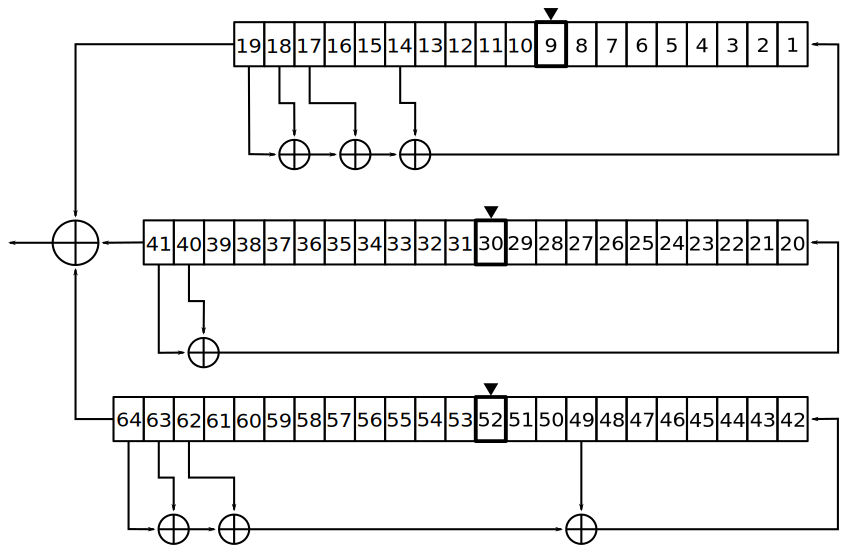
\includegraphics[width=\linewidth]{./a51.eps} 
	\caption{A5/1 generator work scheme} 
	\label{fig:a51gen} 
\end{figure}

The outputs of LFSRs are mixed with linear function, which provides the perfect
corellation immunity. Non-linearity of the equations is achieved by clocking
the registers asynchronously - for each clocking of the whole generator any of
the 3 registers could be clocked or it could retain it's current state.
Register with index $j \in \{1,2,3\}$ will be clocked if the following boolean
function $\chi_j$ becomes 1:

\begin {gather*}
\chi_j = (b_j \equiv majority(b_1,b_2,b_3)); 
\\majority(A,B,C)=(A \wedge B) \vee (A \wedge C) \vee (B \vee C).
\end{gather*}

Here $b_1,b_2,b_3$ denote clocking bits marked at \cref{fig:a5gen} by black
wedges. Conversely, if at some moment $\chi_j=0$, LFSR $j$ won't clock (it will
remain in it's last state).

Generator A5/1 is used in the GSM protocol for high-speed encryption of large
volumes of information with the short secret key. The whole process is split
into 'sessions' about 3,5 hours long. Each session uses it's own 'session key'.
We won't touch on the topic of specialized protocols used in GSM networks to
build and transfer the session key.

Along the message data, GSM protocol sends error correction data for the
message. The message complete with error correction data constitutes a 456 bits
long 'frame', which is further broken down into 4 'bursts' of 114 bits. The
bursts are than encrypted and send over the air. To encrypt a burst the A5/1
generator is initialized with the 64-bit 'local key', that is built using
session key and a natural number called 'the frame number' (FN). After the
encryption of one burst is complete, the frame number is increased by 1. When
FN overflows, the session ends and a new session is initialized (hence the 3,5
session length). FN is always known from the open data transmitted over the
network. 

If the message length is less than 23 bytes, the message would be filled with
fixed pattern padding to 23 bytes. Some GSM technical messages used during the
voice call are fixed length and always padded. As padding is always the same,
and it is encrypted by some local key, we got a typical plain text attack
scenario at hand \cite{MENEZES}. Indeed, the padding plays the role of the
known plaintext, allowing the attacker to get the corresponding keystream
fragment. This vulnerability allows the attacker to get no less than two frames
(912 bits) of the keystream. It was demonstrated in \cite{UNKN1} that the
knowledge of even one local key and FN is enough to efficiently restore the
session key, which makes the decryption of the whole session possible.


The described vulnerability of GSM protocol allows to build some successful
attacks on it, based on the idea of 'advanced brute force'. In particular, the
large-scale preprocessing made possible the creation of the rainbow tables,
which, provided 8 bursts of keystream, allows to determine the session key with
probability in less than a minute with $>85\%$ probability. The tables take
about 2Tb of disk space. This attack is presented in detail in \cite{RAINBOW},
and still stands among the most practical ones. Instead, we will focus on the
idea of an attack that was suggested by Ross Anderson in 1994 in a small essay
on the A5/1 cryptographic strength \cite{ANDERSON}. Next we describe the
essence of the Anderson's attack.


\begin{figure}
	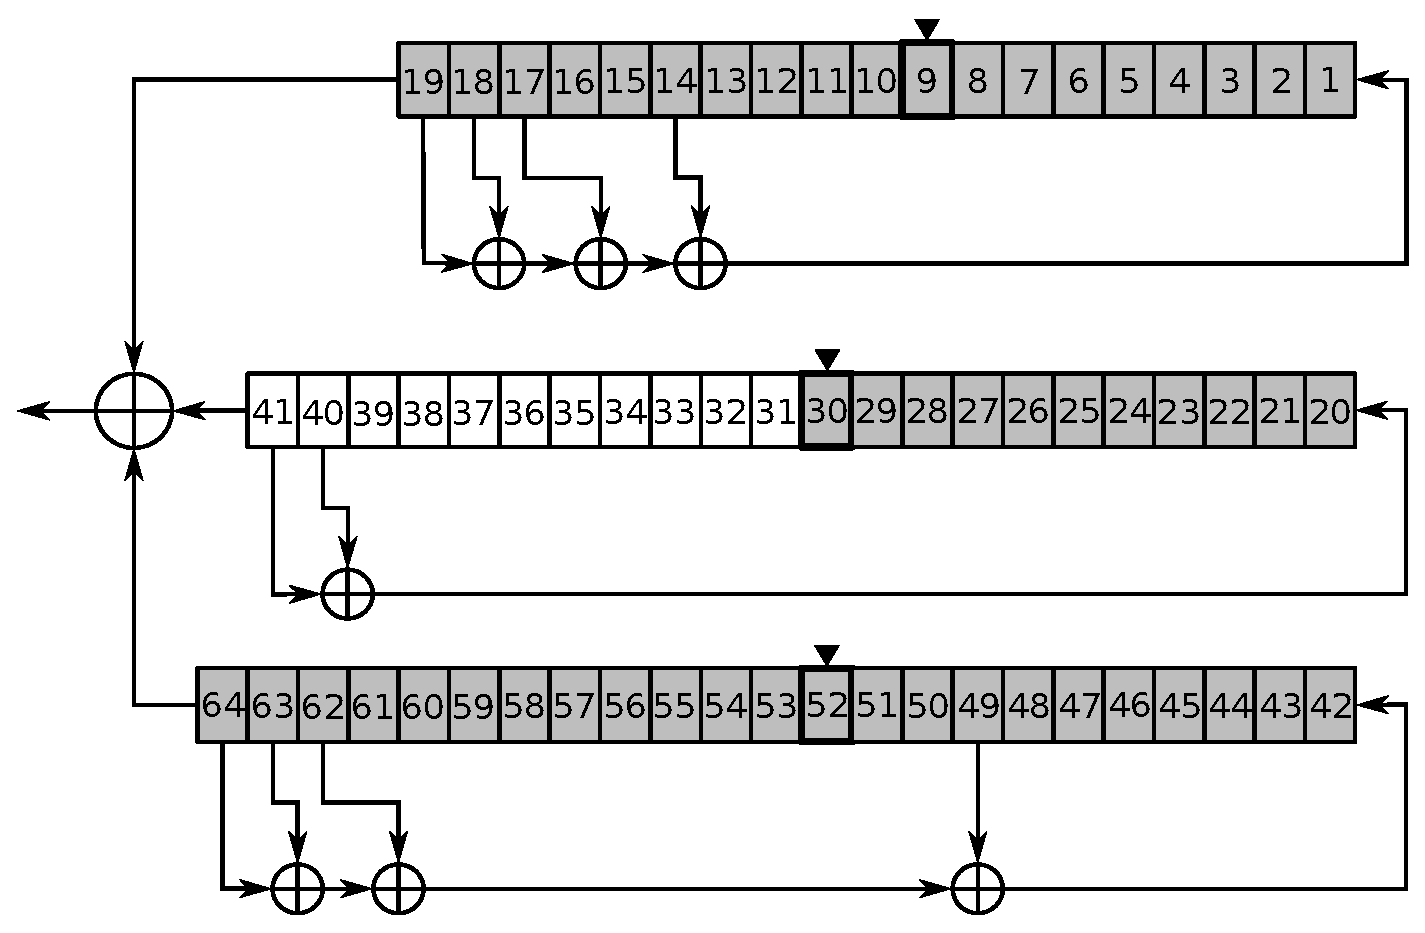
\includegraphics[width=\linewidth]{./a51and.eps} 
	\caption{The set of guessing bits used in Anderson's attack (greyed out).}
	\label{fig:a51and}
\end{figure}


Anderson's attack is a typical example of a 'guess and determine attack' (see
\cite{BARD}). Suppose we know the bits filling the 1st and the 3rd LFSR, and
bits of the 2nd LFSR from the beginning of the register to the clocking bit
(bits 31 to 41, see \cref{fig:a51and}). Next suppose we know 64 bits of the
keystream. Now, as was shown by R. Anderson, 11 unknown bits of the 2nd LFSR
could be figured out without any additional guesses. This happens because the
clocking bits are known (and so is the clocking schedule for the next 11
clockings of the 2nd LFSR), and known are 2 out of 3 XOR-ed LFSR output bits
and the result of the XOR operation (from the keystream). Therefore, one can
efficiently work out the unknown bits of the LFSR 2 one by one, by clocking the
generator and applying XOR operation to corresponding keystream bits and output
bits of LFSRs 1 and 3.

The description of the algorithm of determination of unknown 11 bits of LFSR 2
provided above makes obvious the possibility to mount a brute force attack on
the A5/1 generator over the search space of $2^{53}$. The simplicity of the
algorithm provides an opportunity to implement it on a specialized
computational architecture. One such implementation was built with FPGAs by
authors of \cite{COPAC_1}. In the following sections we describe our
implementation of this attack for a modern GPU.


%%%%%%%%%%%%%%%%%%%%%%%%%%%%%%%%%%%%%%%%%%%%%%%%%%%%%%%%%%%%%%%%%%%%%%%%%%%%%%%
\section{Implementation of the Anderson's Attack in bit-slicing
technique}\label{sec:bitslc}
%%%%%%%%%%%%%%%%%%%%%%%%%%%%%%%%%%%%%%%%%%%%%%%%%%%%%%%%%%%%%%%%%%%%%%%%%%%%%%%

The effeciency of a brute force attack is defined by two parameters: the speed
of checking of the key candidates and the size of the search space. R.
Anderson's idea described above give us a $$2^{53}$$ search space for the A5/1
generator. Instead of using the 'naive' implementation of A5/1 generator, to
speed up the key candidates checking procedure one can opt to use more
sophisticated alternatives. We evaluated the performance of two different fast
implementations of A5/1 generator in \cite{PAVT_2016}. The first one was based
on an idea of precomputation of the states of the registers LFSR 1-3, and
keeping the states in RAM, to use them as the look-up tables. This approach
demonstrated a considerable speed-up against 'naive' implementation. A similiar
method of precomputation of LFSRs was described in \cite{DBLP:conf/fse/BiryukovSW00}. However, in
\cite{PAVT_2016} we found its performance inferior to the second
implementation, that is based on the 'bit-slicing technique'. Next we briefly
describe the idea of this technique, and it's application to Anderson's attack.

Modern general-purpose computational architectures are suboptimal for
implementation of many algorithms. The last operate with bits, while CPUs and
GPUs typically operate with 32-256 bit words. As the result of this
discrepancy, the 'naive' implementation of a cryptographical algorithm won't be
fully using the platform's computational resources. For example, to conduct a
'addition modulo 2' (XOR) operation on 2 boolean arguments, a modern CPU will
position the arguments values into the lowest bits of two 32-bit
general-purpose register (GPR), perform the computation and write the result
into the third 32-bit GPR. In effect, 31 out of 32 bits of GPRs stay idle
during this operation. This problem could be solved by using bitwise operations
that work on GPRs like on boolean vectors - digit by digit. A cryptographical
algorithm could be oftentimes represented as a logical scheme built with the
basic logical gates. Coupled with bitwise operations, this representation
allows the computational platform to apply the algorithm to as many sets of
data, as there are bits in it's GPR (e.g. the platform's register capacity).
This method is called 'SIMD within a register' or the 'bit-slicing' technique.
The first mention of bit-slicing technique applied to cryptographical problem
belongs, seemingly, to E. Biham \cite{BIT_SL}.

Now we describe the main idea of the bit-slicing technique. Consider an
arbitrary total boolean function

\begin{gather*} 
	f:\{0,1\}^n\rightarrow\{0,1\}
\end{gather*}

This function can be represented in the form of the Boolean circuit $C(f)$ over
some complete basis $B$. A common example of such basis is
$B=\{\land,\lor,\neg\}$, but we'll use the basis $B=\{\land,\lor,\neg,\oplus\}$
instead, since it better fits our goals.

Now consider the problem of calculating the arbitrary total boolean function
$f:\{0,1\}^n\rightarrow\{0,1\}$ over all $2^n$ possible inputs. For each input
$X\in\{0,1\}^n$ one can calculate the value of $f$ as a superposition of the
basis functions, according to the scheme $C(f)$. We can now select at least one
fixed order of calculation of basis functions from $C(f)$, that results in
getting the value of $f$. Let $m$ be the number of internal nodes in $C(f)$.
Assuming that the calculation of one basis function takes one processor
instruction, the computation of $f$ over all inputs from $\{0,1\}^n$ will take
$m\cdot2^n$ instructions.

A computational architecture that, in a single instruction execution,
calculates many copies of the same function over many different memory cells,
is called the 'single instruction, multiple data' (SIMD) architecture. When a
modern computational device executes a bitwise logical instruction over its
GPRs, it effectively acts as a SIMD device, individual bits of GPRs playing the
role of the individual memory cells of a SIMD device. The calculation order of
functions in the scheme $C(f)$ always stays the same. This makes it possible to
compute this functions over as many inputs, as there are bits in the device's
GPR.  In effect, if $D$ is the device's GPR capacity, we can simultaneously
walk $D$ instances of the scheme $C(f)$, effectively calculating the value of
$f$ for inputs $X_1,...,X_D$.

Let's examine the arbitrary basis function $g$ with arity 2, and the
corresponding internal node of the scheme $C(f)$. We denote it as $G(x_1,x_2)$,
meaning that it has a single output and two inputs, which values are determined
by boolean variables $x_1,x_2$. Next, collate $g$ with three GPRs denoted
$R_1(g),R_2(g),R_3(g)$, each of which is comprised of $D$ single-bit memory
cells, filled in the following way: 
\begin{itemize} 
\item Register $R_1$ contains $D$ values of the variable $x_1$, corresponding
 to $X_1,...,X_D$; 
\item Register $R_2$ contains $D$ values of the variable $x_2$, corresponding
 to $X_1,...,X_D$;
\item Register $R_3$ contains $D$ values of the function $g$, corresponding to
 matching values of $X_1,...,X_D$.
\end{itemize}
Suppose that all $D$ instances of values of $g$ (matching the corresponding
values of $x_1$ and $x_2$) can be computed as a result of a single bitwise
instruction applied to register $R_1(g),R_2(g)$, while their result is put into
register $R_3(g)$.  If this fact is holding true for every basis function in
the scheme $C(F)$, the computation of $f$ for every input from $\{0,1\}^n$ will
require $m\cdot\frac{2^n}{D}$ instructions. This is the key idea of the
bit-slicing technique \cite{fig:bitsl}.


\begin{figure} 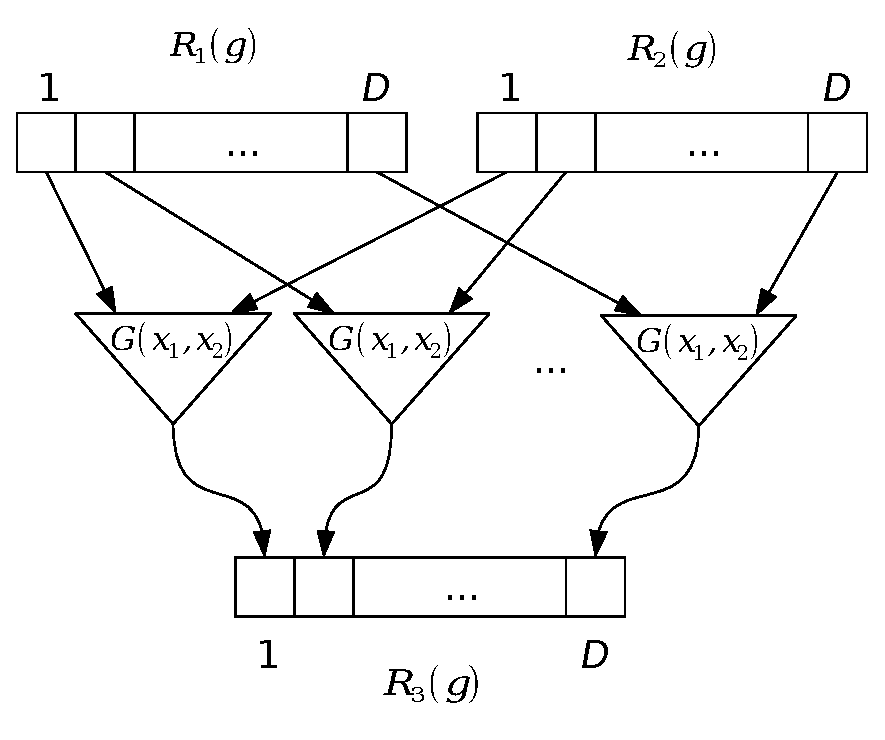
\includegraphics[width=\linewidth]{./bitslice.eps}
	\caption{Simultaneous computation of $D$ instances of scheme $C(f)$ with
	bit-slicing technique} \label{fig:a51gen} 
\end{figure}

We will call the process of computation of the function $f$ on a single input
from $\{0,1\}^n$ a "thread", by analogy with the computational threads in a
SIMD device. So, with the use of bit-slicing technique, it takes $m$
instructions to complete the computation of $D$ threads.

Now we describe the details of bit-slicing implementation of the A5/1
generator. Suppose that a computational device is able to calculate $D$
instances of any function from the basis $B=\{\land,\lor,\neg,\oplus\}$. Each
of $n\in\{1,...,64\}$ cells of LFSR 1-3 gets a matching word $W_n\in\{0,1\}^D$:

\begin{gather*} 
	LFSR1:W_1,...,W_{19}; 
	\\LFSR2:W_{20},...,W_{42}; 
	\\LFSR3:W_{43},...,W_{64}.
\end{gather*}

In a bit-slicing technique, the shift of the LFSR register (LFSR 1 in this
example) will take the following form: 
\begin{gather*} 
	W`_1=W_{19} \oplus W_{18} \oplus W_{17} \oplus W_{14}, 
	\\W`=W_{n-1}, n \in \{2,...,19\},
\end{gather*}
where $\oplus$ is the bitwise addition modulo 2 of boolean vectors of length
$D$ operator. The calculation of the keystream bit will look like:
\begin{gather*} 
	W_{out}=W_{19} \oplus W_{41} \oplus W_{64}.
\end{gather*}

The conditional clocking is somewhat more complex to implement in a bit-slicing
technique. First, to know if the LFSRs should be shifted or not, one needs to
calculate the corresponding clocking flags $F_1,F_2,F_3$ using the majority
function: 
\begin{gather*} 
	W_{maj}=maj(W_8,W_{30},W_{52})=(W_9 \wedge W_{30}) \vee (W_9 \wedge W_{52})
	\vee (W_{30} \vee W_{52}), \\F_1 = W_9 \oplus {\neg W_{maj}}, \\F_2 =
	W_{30} \oplus {\neg W_{maj}}, \\F_3 = W_{52} \oplus {\neg W_{maj}},
\end{gather*} 
(all operations are bitwise operations on the vector of the length $D$).

To implement the conditional clocking of a LFSR one can use the bitwise
counterpart of the "bitselect" function of arity 3: 
\begin{gather*} a,b,c \in \{0,1\}; \\ BS(a,b,c) = \left\lbrace
	\begin{array}{ll} b,a=1, \\ c,a=0.
	\end{array} \right.
\end{gather*} 

If the computational architecture lacks the hardware implementation of this
function, it can be emulated with the usage of the standard bitwise functions
corresponding to the functions of the basis $B$ (example for LFSR 1):
\begin{gather*} BS(a,b,c) = (a \wedge b) \vee (\neg a \wedge c).
\end{gather*}

Clocking the LFSR 1 with the use of $BS(a,b,c)$ and corresponding flag $F_1$
looks the following way:
\begin{gather*} 
	W'_1 = BS(F_1, (W_{19} \oplus W_{18} \oplus W_{17} \oplus W_{14}), W_1);
	\\W'_n = BS( F_1, W_{n-1}, W_n), n \in \{2,..,19\}.
\end{gather*}

Some important details about the bit-slicing implementation of the Anderson's
attack should be covered still. The Anderson's attack follows 2 stages:
\begin{enumerate} 
	\item Calculating the values of 11 bits of LFSR 2 lying left of the
	 clocking bit with the information from the remaining 53 bits (guessed) and
		the keystream (known).
	\item Clocking the generator as normal to check if the guessed filling of
	 the generator matches the known keystream.
\end{enumerate}

The irregular clocking of the A5/1 generator makes it generally impossible to
predict how many clockings of the whole generator (bits of keystream) would be
needed to shift LFSR 2 11 times to complete the Stage 1 of the attack.
Therefore, we again put to use the bitselect function to implement the split of
the attack into 2 stages. Since each individual thread should be able to stay
in a stage and advance to the next stage independent of other threads, we
introduce the special boolean vector $\phi = (\phi_1,...,\phi_D)$, called the
"attack stage flag". The thread with number $i, i \in \{1,...,D\}$ being in the
Stage 1 of the attack corresponds to $\phi_i = 0$, and the Stage 2 of the
attack corresponds to $\phi_i=1$. Let $y_1,...,y_{64}$ be the bits of the
keystream analyzed. Now the clocking of the LFSR 2 considers the stage of the
attack through the usage of the attack stage flag: \begin{gather*} W^\ast_{41}
	= BS(\phi, W_{41},(y \oplus W_{19} \oplus W_{64}));\\W'_{20} =
	BS(F_2,(W^\ast_{41} \oplus W_{40}), W_{20});\\W'_n = BS(F_2,W_{n-1},W_n), n
	\in \{20,...,41\}. 
\end{gather*}

Here $W^\ast_{41}$ is a helper vector holding temporary data. $y$ is the
current bit of the keystream, in the form of a vector consisting of $D$ copies
of $k$-th bit of the keystream. In effect, Stage 1 of the attack's goal is to
calculate the last bit of the LFSR 2 from known keystream bits and known
(guessed) last bits of the LFSRs 1 and 3. At the Stage 2 the last bit of the
LFSR 2 is known and the whole generator scheme is clocked as normal. For the
$i$-th thread the attack stage flag $\phi_i$ is set to 1 after the thread's
instance of LFSR 2 was shifted 11 times. To count the number of LFSR 2 shifts
on a per-thread basis, the bit-slicing implementation of an incremental counter
is used.

The Anderson's attack algorithm described above was realized on an NVIDIA GPU
with the use of CUDA SDK 8.0 \cite{CUDA}. The comparison of the performance of
a GPU to a CPU in execution of bit-slicing and LFSR precomputation-based
\cite{DBLP:conf/fse/BiryukovSW00} implementations of Anderson's attack is shown in
\cite{tab:gpuspeed}.

\begin{table} \caption{(LOP3.LUT is a special instruction that implements
	arbitrary bitwise arity 3 functions in hardware. We use it as a substitute
	for the "bitselect" instruction.)} 
	\label{tab:gpuspeed} Performance of the different implementations of the
	Anderson's attack (search space is $2^{53}$) on a CPU and a GPU, measured
	in millions of key checks per second.  
	\begin {center} 
	\begin{tabular} {| l | l | l |} \hline Computational device & Bit-slicing &
		LFSR precomputation \cite{DBLP:conf/fse/BiryukovSW00} \\ \hline CPU Intel Core I7 930 & 37 & 7
		\\ \hline GPU NVIDIA GTX 1050 Ti & 9180 & 483 \\ \hline GPU NVIDIA GTX
		1050 Ti (LOP3.LUT) & 11950 & - \\ \hline
	\end{tabular}
\end {center}
\end{table}

Data provided in the \Cref{tab:gpuspeed} tells us that even one mid-range
consumer GPU is enough to make the Anderson's attack run time practical (it
will take around 250 hours). A modern computational cluster outfitted with GPUs
will complete the attack in mere minutes or less. The Anderson's attack's
advantage over the rainbow-tables attack \cite{RAINBOW} is the former's ability
to restore the secret key from 64 bits of keystream with the 100\% probability.
It's advantge over the attack described in \cite{COPAC_1} is in a usage of a
consumer-grade off-the-shelf hardware.


%%%%%%%%%%%%%%%%%%%%%%%%%%%%%%%%%%%%%%%%%%%%%%%%%%%%%%%%%%%%%%%%%%%%%%%%%%%%%%%
\section{Implementation of the Anderson's Attack in a volunteer computing
project}\label{sec:boinc}
%%%%%%%%%%%%%%%%%%%%%%%%%%%%%%%%%%%%%%%%%%%%%%%%%%%%%%%%%%%%%%%%%%%%%%%%%%%%%%%
In order to solve 10 cryptanalysis problems for the A5/1 keystream generator we
launched the volunteer computing project AndersonAttack@home. The client (computing)
application of this project is based on the CUDA implementation, which was
described in the previous section.

Volunteer computing \cite{DBLP:conf/ccgrid/AndersonF06} is a type of distributed computing \cite{Foster:1995:DBP:527029} which uses computational resources of PCs (hosts) of private persons called volunteers. 
Each volunteer computing project is designed to solve one or several hard scientific problems. When PC is
connected to a project, all calculations are performed automatically and
do not inconvenience user since only idle PC resources are used.

Each volunteer computing project consists of the following basic parts: server
daemons, database, web site and client application. Daemons include
\textsc{work generator} (it generates tasks to be processed), \textsc{validator}
(it checks the correctness of the results received from volunteer's PCs) and
\textsc{assimilator} (aimed at processing correct results). A client application should
have versions for the widespread computing platforms.  One of attractive
features of volunteer computing is its low cost --- to maintain a project one
only needs a dedicated server working 24/7.

AndersonAttack@home is based on BOINC (Berkley Open Infrastructure for Network
Compuitng \cite{Anderson:2004:BSP:1032646.1033223}), which is the most popular platform for
volunteer computing. Each BOINC-based project is separate, but any private
person can take part in arbitrary project with the help of the standard BOINC
manager. This manager allows users to change projects priority and to
regulate the mode of PC using. 

BOINC provides a form of redundant computing.  According to this, several (at
least 2) similar tasks are created for each workunit. These tasks are processed
on multiple hosts, the results are compared on a project server by validator,
and are accepted only when a 'consensus' is reached. The sufficient number of
successful results is called a 'quorum'. If for a particular workunit results
of tasks are nonsimilar, then new tasks must be created and sent. The scheme of
a BOINC-based project with the quorum of 2 is shown on Fig.~\ref{fig:boinc}.

%\begin{figure}
%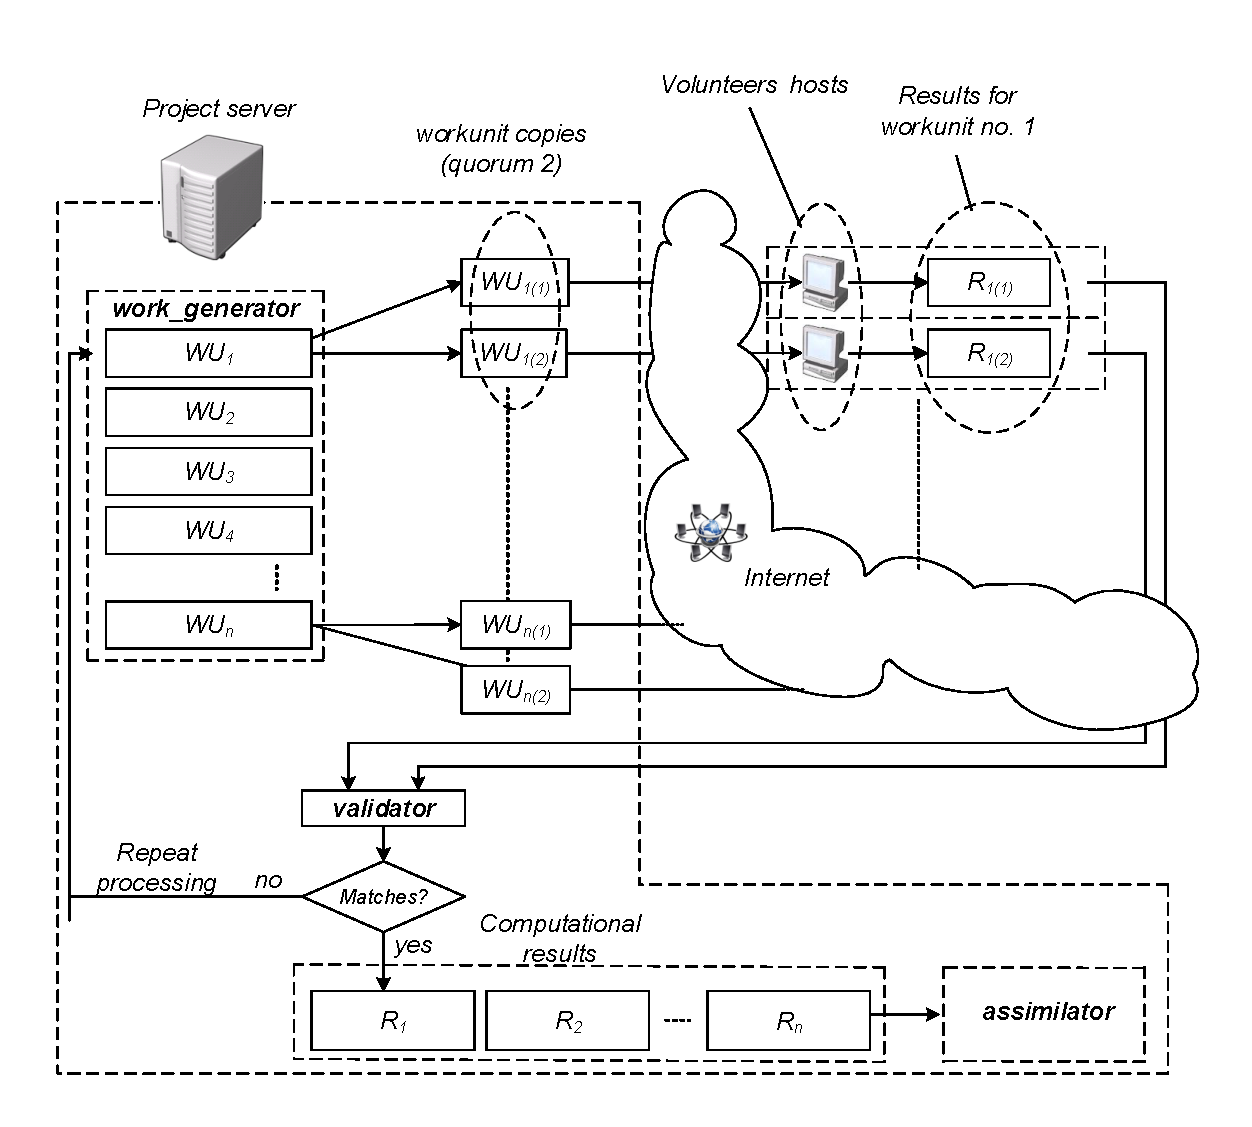
\includegraphics[width=\linewidth]{./BOINC_project_scheme.eps}
%	\caption{The scheme of a BOINC-based project with the quorum of 2} 
%	\label{fig:boinc} 
%\end{figure}

In the first stage of our experiment, a family of workunits was generated on 
the project server. In each workunit values of 12 out of 53 cells of the A5/1 generator (see the previous section) 
were fixed. Thus, 40960 workunits were generated for 10 cryptanalysis problems in total. Usually, the
value of deadline for workunits in BOINC projects is equal to 10-14 days. In
our project, we used a deadline of 1 day, because the experiment was quite
small. In the next stage all generated workunits were processed in a desktop
grid formed by project's hosts. This took about 7 days. As a result, solutions
for all considered problems were successfully found (see Table~\ref{tab:keys}). It should be noted, 
that we found collisions for 7 out of 10 problems (5 of them have 1 collision, each of other 2 problems has 2
collisions).

\begin{table} 
\caption{} 
\label{tab:keys} Original secret keys and collisions of the
	generator A5/1 (in hexadecimal format) which were found in
	AndersonAttack@home.
	\begin {center} 
		\begin{tabular}
			{| l | l | l |}
			\hline
			Instance & Keystream & Secret key \\ \hline
			1 & 0x770c0410869366f1 & original 0x11b8e4340276c4ee \\
			  &                    & collision 1 0x42634f3266d302a3 \\ \hline
			2 & 0xae9590560c26e9ed & original 0x4c656fd73e59ab9b \\
			  &                    & collision 1 0xcf23e4722e3cfb68 \\ \hline
			3 & 0xdd4b3ab7f6cf8224 & original 0x09429d158555f4b3 \\
			  &                    & collision 1 0x09429d158553e967 \\
			  &                    & collision 2 0x40e5f2c8128a1781 \\ \hline
			4 & 0x93cd42d97eb75fd9 & original 0xfa386a338355aafd \\
			  &                    & collision 1 0xf9e81096bb4d0aad \\ 
			  &                    & collision 2 0xf9e81096bb4a8556 \\ \hline
			5 & 0x925e423c98121152 & original 0xe5cf81035ce5fbe2 \\ \hline
			6 & 0x3b3464bd6e377b87 & original 0x9625e9d810b46248 \\
			  &                    & collision 1 0xf5aa1be2d6c36e18 \\ \hline
			7 & 0x0367d29121dd1677 & original 0xd1b8b06086edf162 \\ \hline
			8 & 0x6b49230b7fc0249d & original 0xbe81a896968c486b \\ \hline
			9 & 0xc65847556752d14c & original 0xb6f65d2855a211c0 \\ 
			  &                    & collision 1 0xb6f65d2855a508e0 \\ \hline
			10& 0x07bb7f83d26072ec & original 0x122a1a2955286b9f \\ 
			  &                    & collision 1 0xd5151aaa50490012 \\ \hline
		\end{tabular}
	\end {center}
\end{table}


According to BOINC statistics, 143 active hosts of 90 volunteers participated
in the experiment. Here by 'active' we mean a host which correctly processed
at least one task. Active volunteer has at least one active host. It should be
noted, that there is only 1 volunteer from Russia in top-10 project's volunteers list
(formed according to the amount of calculations), the most of them are from United
States (4 persons). In top-10 list of teams there is only one team from Russia
too.

%%%%%%%%%%%%%%%%%%%%%%%%%%%%%%%%%%%%%%%%%%%%%%%%%%%%%%%%%%%%%%%%%%%%%%%%%%%%%%%
\section{Related works.}\label{sec:related}
%%%%%%%%%%%%%%%%%%%%%%%%%%%%%%%%%%%%%%%%%%%%%%%%%%%%%%%%%%%%%%%%%%%%%%%%%%%%%%%

As was noted before, at the time of writing of our article the A5/1 algorithm
remains one of the most popular research subjects among cryptography
specialists, along with DES and RSA algorithms. The exact authorship of this
algorithm is unknown, but some experts argue that chances are high that its
creation should be attributed to a French special agencies. Numerous sources
describe the events that led to its structure leaking to general public. In
fact, its internal workings were already known to research community in 1994:
R. Anderson's note (a mailing list message) written in that period was one of
the first works on A5/1 cryptanalysis. The complete knowledge of A5/1 were
acquired in 1999 as a result of a reverse engineering of a mobile phone.

Earlier we mentioned Anderson's attack (described by Ron Anderson in a short
note in 1994 \cite{ANDERSON}) was the first attack on A5/1 with compexity less
than that of a trivial brute-force walk over the whole keyspace. Shortly
afterwards J. Golic suggested the ``Alleged'' attack on the A5/1, based on a
linearization of the equations describing A5/1 \cite{Golic1997}. The Golic's attack
estimated complexity is $C \cdot 2^{40}$, where $C$ denotes the complexity of
solving the system of linear equations over $GF(2)$ with a very substanial
number of dimensions. The next widely known attack on the A5/1 was presented in
\cite{DBLP:conf/fse/BiryukovSW00}. To speed up the A5/1 algorithm its authors used the technique of
precomputation of LFSRs we mentioned in \Cref{sec:bitslc}. It's worth to note
that the attack presented in \cite{DBLP:conf/fse/BiryukovSW00}, along with those presented in
\cite{Biham2000,DBLP:journals/tit/EkdahlJ03,Barkan2008}, require substanial
lengths of known keystream (several seconds at best). These attacks can be
deemed realistic, but they do not demonstrate vulnerability of the GSM security
protocols as evidently, as those belonging to the ``advanced brute force'' class,
that we will discuss below. For the rest of the section we consider an attack
practical if its real-life implementation is able to persistently find the
secret key by analyzing no more than 2 frames (912 bits) of a keystream, the
amount that could always be extracted from a call in a GSM network by
exploiting the protocol vulnerability described in \Cref{sec:alg}.

It seems that the first practical attack (``practical'' in a sense we established
above) was presented in \cite{Guneysu:2008:CC:1446228.1446266}. It's authors implemented the optimized
variant of the Anderson's attack on a specialized computational device of their
own design, assembled from 120 ``Xilinx Spartan 3'' FPGAs. The authors state
\cite{Guneysu:2008:CC:1446228.1446266} that the attack took about 6 hours to complete. It's worth
mentioning that the COPACOBANA architecture was used for cryptanalytical
research of several other ciphers, e.g. DES \cite{COPAC_2}.

The first estimates of the time required for the cryptanalysis of A5/1 on a
computational cluster in the form of a boolean satisfiability problem (SAT)
\cite{HANDBOOK} were presented in \cite{PACO-2008}. SAT-based cryptanalysis is
considered a perspective direction of cryptanalysis that seems to be on the
rise for the last decade. It operates within a paradigm that the
cryptanalytical problem could be effeciently represented in the form of a SAT
problem. This could be achieved with the help of special translators such as
\cite{CRYPTOL}, \cite{URSA}, \cite{TRANSALG}. After the problem was translated
to a SAT form, it can be efficiently solved by modern SAT algorithms that could
run in a distributed computing environment. The cryptanalysis time of A5/1
estimated in \cite{PACO-2008} was realistic, but since the exclusive usage of
the whole computational cluster for prolonged period of time was not an option,
the actual attack was performed a year later in a specialized grid-system
\cite{TRUDY_ISA}. In the following years these results were improved - the
search space of $2^{31}$ SAT instances was processed completely and collisions
(different secret keys generating the same keystream) have been found
\cite{SZBP}. At the same period it became apparent that the organizational
requirements of this kind of cryptographical attack fits well into the ideology
of volunteering computing projects \todo{cite what?}. To bring this line of
thought to life in 2012 SAT@home \cite{SATHOME} volunteering computing project
was incepted. Through 4 years of it's activity a number of hard combinatorial
problems were solved within the SAT paradigm. Among those were several dozens
of cryptanalysis of A5/1 generator problems (only one burst - 114 bits of
keystream - was used each time). These results were published in
\cite{PACT_2015}, \cite{SPRINGER}.

The work \cite{COPAC_2} included the estimates of creation time and disk space
that would be required to create the rainbow-tables that would make possible to
'break' the A5/1 on an average PC in several minutes. \cite{COPAC_2} estimated
these to occupy about 7 Tb of disk space. "The A51 Cracking Project" put the
significantly more compact (2 Tb) tables into public domain at the end of 2009
\todo {cite what?}. By analysing 2 frames (912 bits) of known keystream with
the help of this tables one can restore the secret key with probability of
success over 85\%. This method of cryptanalysis of the A5/1 algorithm could be
assumed to be the most practical. The fact that it does not provide 100\%
guarantee of success from analysis of 2 frames does not matter in real
circuimstances, where much longer samples of keystream are available to the
attacker. It should be noted that if the tables are lost, it will require a
vast amount of computational resources to generate them again.

Finally, the attack we presented in this paper does not lose on the practical
side to the rainbow-tables attack, because it allows to complete the
cryptanalysis with 100\% success rate in a period of several hours in a small
volunteering computation project. Moreover, the attack requires only 64 bits of
known keystream. Volunteering computing projects are rising in popularity and
publicity in the last years, so any "hot" problem (like a cryptanalysis of one
of the most commonly used ciphers) immediately gets volunteers attention.

As a conclusion, we would like to express the hope that the efficiency of our
implementation of attack on A5/1 generator will serve as yet another strong
argument against the usage of this algorithm in the transfer of sensible data
through GSM networks.

\section*{Acknowledgment}
The research was funded by Russian Science Foundation (project No. 16-11-10046). The authors would like to thank Stepan Kochemazov for helpful discussions and valuable comments.

%%%%%%%%%%%%%%%%%%%%%%%%%%%%%%%%%%%%%%%%%%%%%%%%%%%%%%%%%%%%%%%%%%%%%%%%%%%%%%%
\bibliographystyle{splncs03}
\bibliography{pact2017_bulavintsev_ref}
%%%%%%%%%%%%%%%%%%%%%%%%%%%%%%%%%%%%%%%%%%%%%%%%%%%%%%%%%%%%%%%%%%%%%%%%%%%%%%%

\end{document}
